\documentclass[aspectratio=1610, handout]{beamer}
\usepackage[utf8]{inputenc}
\usepackage{ragged2e}
\usepackage{xcolor}
\usepackage[italian]{babel}
\usetheme[progressbar=frametitle,titleformat=smallcaps]{metropolis}
\setbeamertemplate{frame numbering}[fraction]
\setbeamercovered{dynamic}
\definecolor{rosso}{RGB}{255, 0, 0}
\definecolor{giallo}{RGB}{254,212,23}
\hypersetup{colorlinks=true,linkcolor=black,urlcolor=rosso}
\setbeamercolor{palette primary}{fg=black, bg=giallo}
\setbeamercolor{background canvas}{bg=white}
\setbeamercolor{normal text}{fg=black}
\setbeamercolor{progress bar}{fg=rosso}
\setbeamercolor{framesubtitle}{fg=rosso}
\setbeamercolor{normal text .dimmed}{fg=giallo}
\setbeamercolor{block title alerted}{fg=rosso, bg=giallo}
\setbeamerfont{caption}{size=\tiny}
\setbeamerfont{caption name}{size=\tiny}
\setlength{\abovecaptionskip}{0pt}
\makeatletter
\metroset{block=fill}
\setlength{\metropolis@progressinheadfoot@linewidth}{1pt} 
\setlength{\metropolis@progressonsectionpage@linewidth}{1pt}
\setlength{\metropolis@titleseparator@linewidth}{1pt}

\makeatother

\title{RETI INFORMATICHE}
\subtitle{introduzione alle reti informatiche e alle tipologie di rete}
\date{}
\institute{\textit{
        Fonti:
        \begin{itemize}
            \item[-] \href{https://it.wikipedia.org/wiki/Rete_di_computer}{Wikipedia}
            \item[-] \href{https://www.cappellieditore.it/testi/skills-box/}{SkillsBox}
        \end{itemize}
    }
}

\begin{document}

\begin{frame}[plain, noframenumbering]
    \titlepage
\end{frame}

\section{DEFINIZIONI}

\begin{frame}{RETE DI TELECOMUNICAZIONI}
    \begin{alertblock}{DEFINIZIONE}
        \begin{minipage}{0.98\linewidth}
            \justifying
            Una \textbf{rete di telecomunicazioni} è un insieme di dispositivi e dei loro collegamenti (fisici o logici),
            che consentono la trasmissione e la ricezione di informazioni di qualsiasi tipo tra due o più utenti situati 
            in posizioni geograficamente distinte, effettuandone il trasferimento attraverso un qualsiasi mezzo di comunicazione.
        \end{minipage}
    \end{alertblock}
\end{frame}

\begin{frame}{RETE INFORMATICA}
    \begin{alertblock}{DEFINIZIONE}
        \begin{minipage}{0.98\linewidth}
            \justifying
            Una \textbf{rete di computer} o \textbf{rete informatica} è un tipo di rete di telecomunicazioni a commutazione di pacchetto; 
            è caratterizzata da un insieme di dispositivi hardware (\textbf{nodi}) collegati l'uno con l'altro da appositi canali 
            di comunicazione (\textbf{link}), tali da fornire un servizio di comunicazione che permette la condivisione di dati e la 
            comunicazione tra più utenti o dispositivi terminali (\textbf{host}): i dati vengono trasmessi e trasferiti sotto forma di pacchetti 
            dati, il tutto regolato da precisi \textbf{protocolli di rete}.
        \end{minipage}
    \end{alertblock}
\end{frame}

\section{TIPOLOGIE DI RETE}

\begin{frame}{TIPOLOGIE DI RETE}
    \begin{columns}
        \column{.5\textwidth}
            \justifying
            \textbf{PAN (Personal Area Network)} \\
            Rete personale che collega dispositivi entro una distanza molto limitata (circa 10 metri). Tali 
            dispositivi possono scambiarsi informazioni tramite differenti mezzi di trasmissione dati, in genere 
            tramite Bluetooth.\\
            \bigskip
            \tiny{\textbf{curiosità}}\\
            \tiny{\href{https://www.ilpost.it/2014/12/31/bluetooth/}{Perchè si chiama "Dente Blu"?}}
        \column{.5\textwidth}
            \begin{figure}
                
\includegraphics[width=\linewidth]{img/pan.png}
                \caption{{creata con \href{https://www.canva.com/}{Canva}}}
            \end{figure}
    \end{columns}
\end{frame}

\begin{frame}{TIPOLOGIE DI RETE}
    \begin{columns}
        \column{.5\textwidth}
            \justifying
            \textbf{LAN (Local Area Network)} \\
            Rete locale che copre un'area (generalmente privata) ristretta, come una casa, un ufficio, un edificio 
            o un complesso di edifici adiacenti (ad esempio una scuola). I nodi di rete sono connessi tra loro tramite mezzi 
            di comunicazione \textbf{wireless} o \textbf{wired}.\\
        \column{.5\textwidth}
            \begin{figure}
                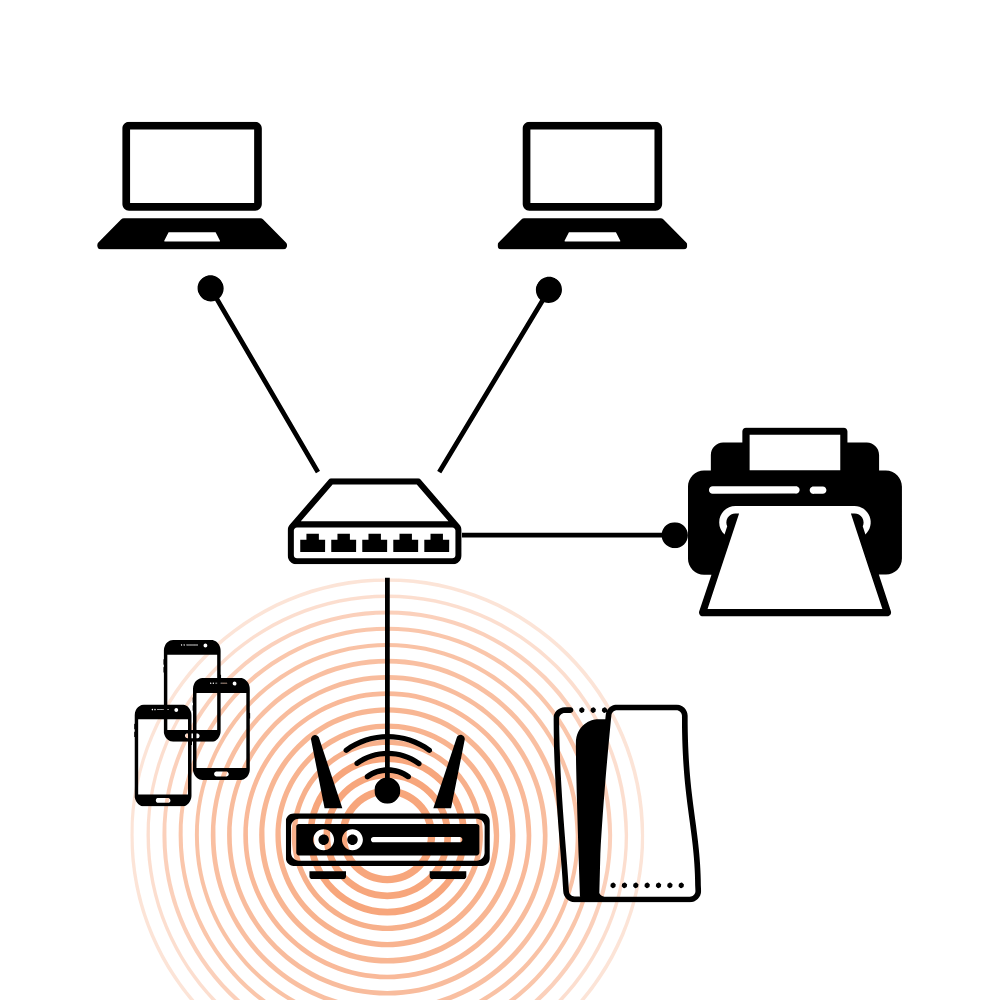
\includegraphics[width=\linewidth]{img/lan.png}
                \caption{{creata con \href{https://www.canva.com/}{Canva}}}
            \end{figure}
    \end{columns}
\end{frame}

\begin{frame}{TIPOLOGIE DI RETE}
    \begin{columns}
        \column{.5\textwidth}
            \justifying
            \textbf{WLAN (Wireless Local Area Network)} \\
            Rete locale (molto diffusa nelle abitazioni private), \textbf{variante della LAN}, caratterizzata 
            dall'assenza di cavi di collegamento. Tra i nodi la connessione avviene tramite soli canali \textbf{wireless},
            in genere tramite \textbf{Wi-Fi}.\\
            \bigskip
            \tiny{\textbf{curiosità}}\\
            \href{https://accademiadellacrusca.it/it/consulenza/il-wifi-o-la-wifi-limportante-alla-fine-\%C3\%A8-che-funzioni/1247}{Il Wi-Fi o la Wi-Fi?}
        \column{.5\textwidth}
            \begin{figure}
                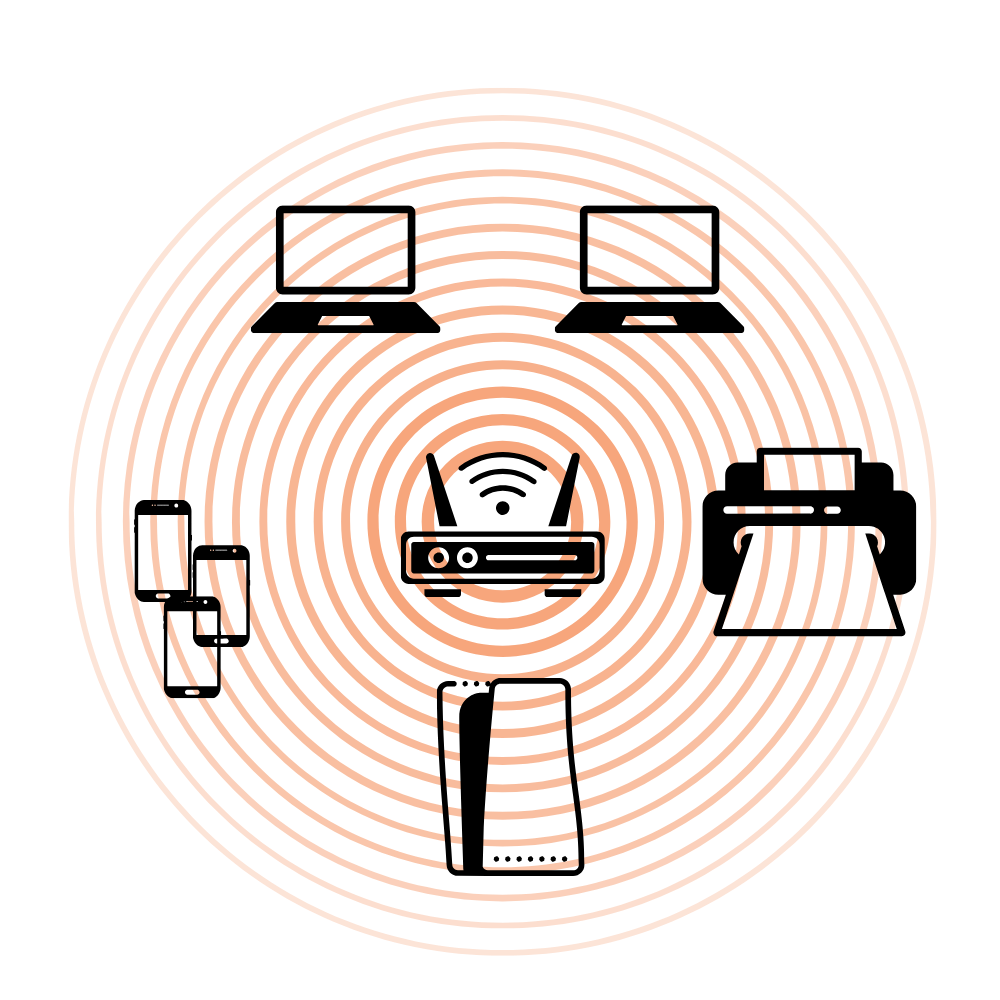
\includegraphics[width=\linewidth]{img/wlan.png}
                \caption{{creata con \href{https://www.canva.com/}{Canva}}}
            \end{figure}
    \end{columns}
\end{frame}

\begin{frame}{TIPOLOGIE DI RETE}
    \begin{columns}
        \column{.5\textwidth}
            \justifying
            \textbf{MAN (Metropolitan Area Network)} \\
            Rete geografica metropolitana che copre un'area urbana o una città. Un esempio è la rete che collega 
            in un'università diversi uffici, facoltà e dipartimenti dislocati nella stessa città, ma in zone 
            differenti.
        \column{.5\textwidth}
            \begin{figure}
                
\includegraphics[width=\linewidth]{img/man.png}
                \caption{{creata con \href{https://www.canva.com/}{Canva}}}
            \end{figure}
    \end{columns}
\end{frame}

\begin{frame}{TIPOLOGIE DI RETE}
    \begin{columns}
        \column{.5\textwidth}
            \justifying
            \textbf{WAN (Wide Area Network)} \\
            Rete geografica che si estende all'interno di una regione o di un intero stato. Solitamente è utilizzata 
            per collegare più reti MAN tra loro, in modo da rendere possibile la comunicazione tra nodi di rete 
            appartenenti a centri urbani differenti.
        \column{.5\textwidth}
            \begin{figure}
                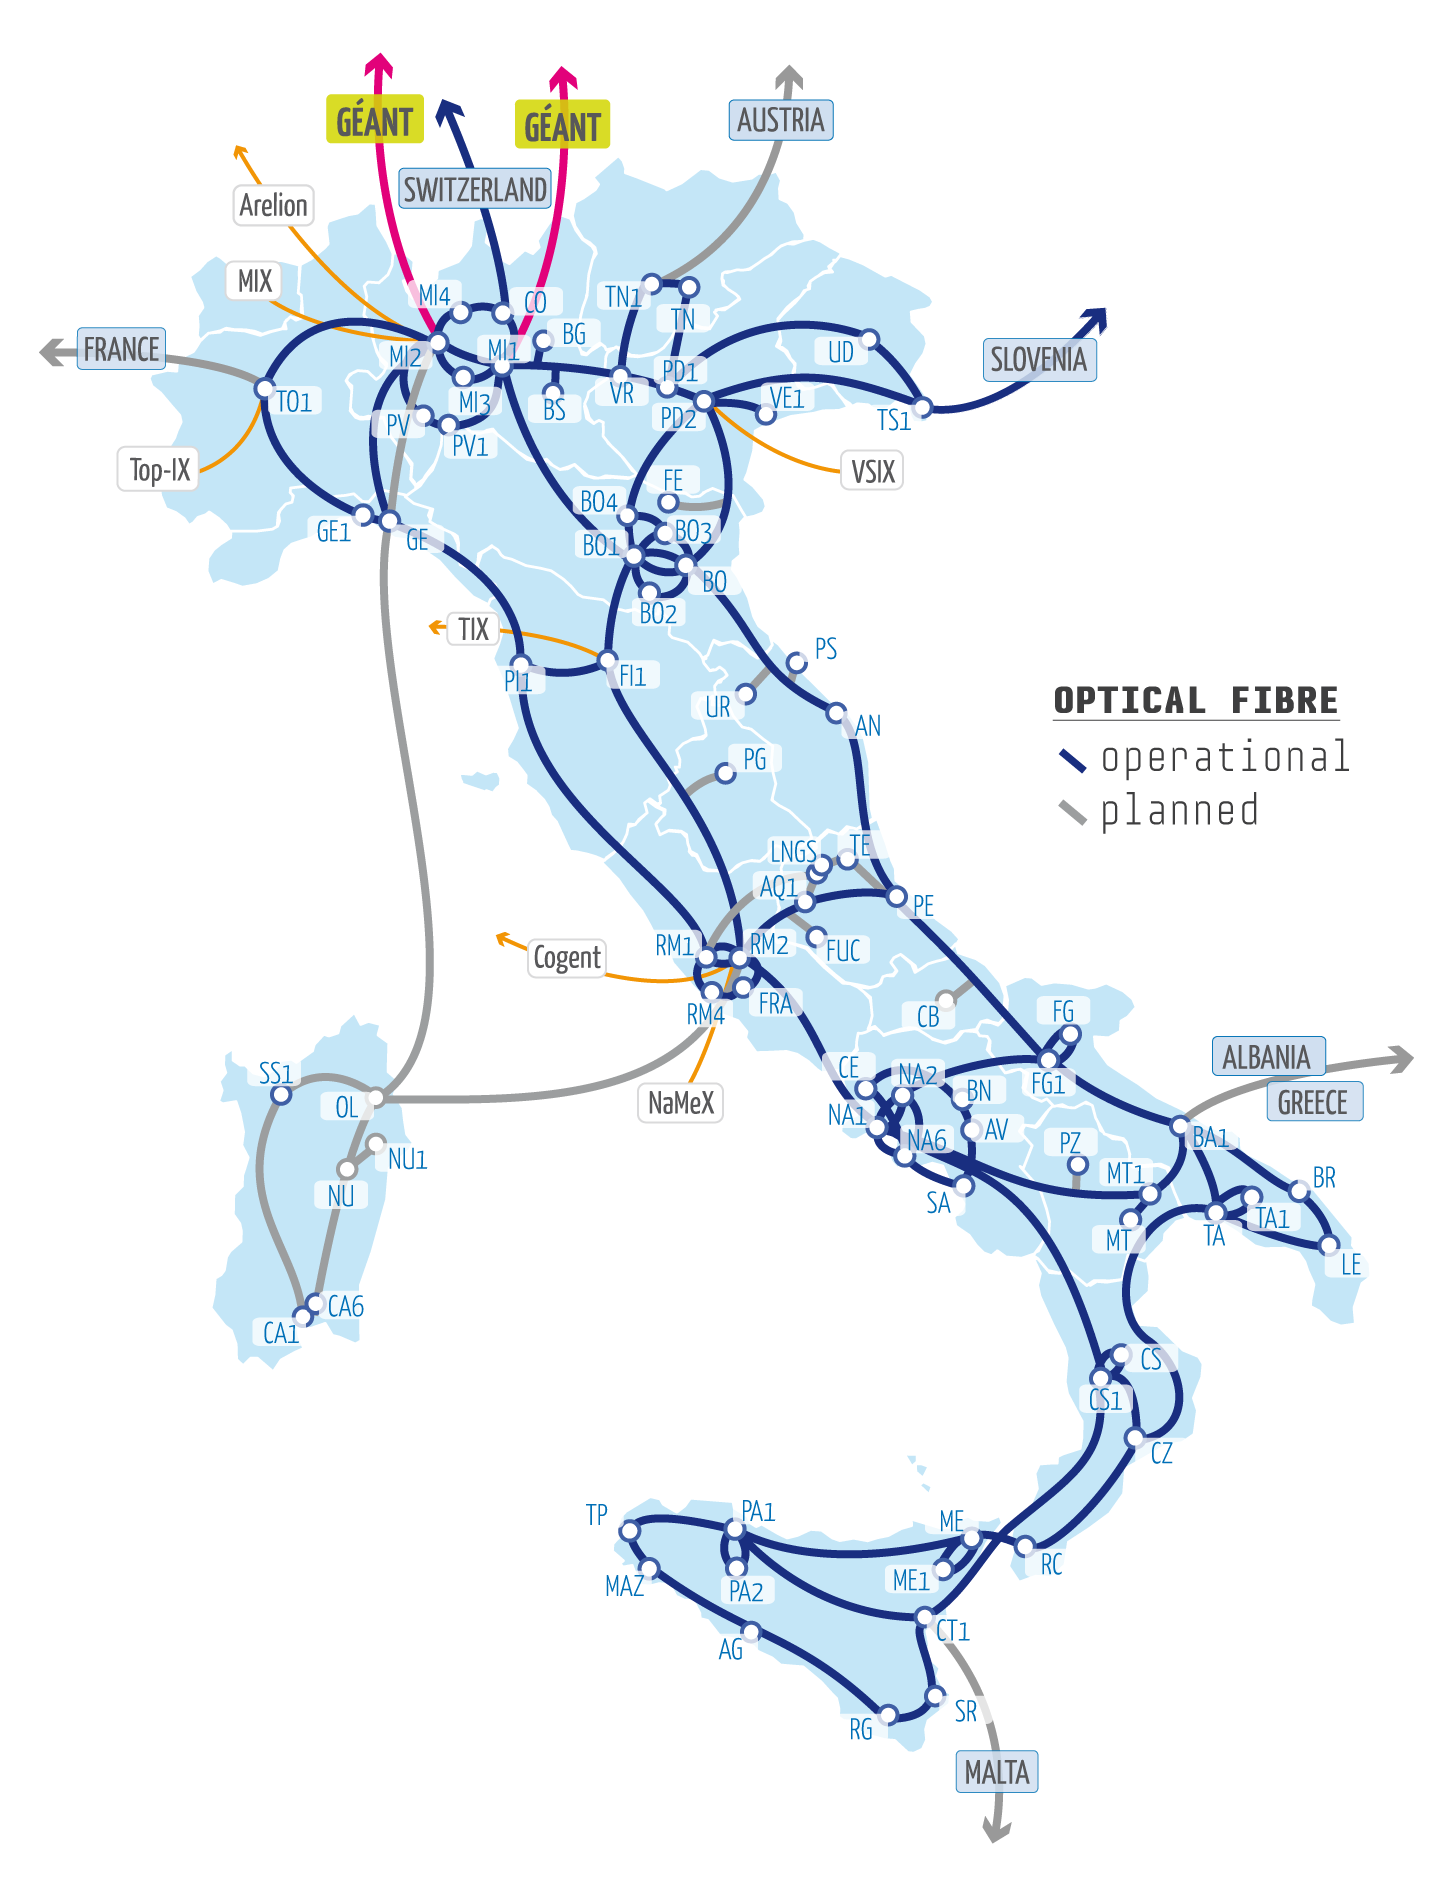
\includegraphics[width=0.77\linewidth]{img/wan.png}
                \caption{{fonte \href{https://www.garr.it/it/infrastrutture/rete-nazionale/mappa-della-rete}{Consortium GARR}}}
            \end{figure}
    \end{columns}
\end{frame}

\begin{frame}{TIPOLOGIE DI RETE}
    \begin{columns}
        \column{.5\textwidth}
            \justifying
            \textbf{GAN (Global Area Network)} \\
            Rete globale che collega tra loro tutte le precedenti reti di dimensione minore, e in cui i nodi sono 
            dislocati in tutti i continenti del pianeta. La trasmissione dei dati può avvenire con differenti modalità, 
            \textbf{sia wired che wireless}. L'esempio più famoso di rete GAN è \textbf{Internet}.\\
            \bigskip
            \tiny{\textbf{curiosità}}\\
            \tiny{\href{https://maps.agcom.it/}{Mappa AGCOM per l'accesso a Internet}}
        \column{.5\textwidth}
            \begin{figure}
                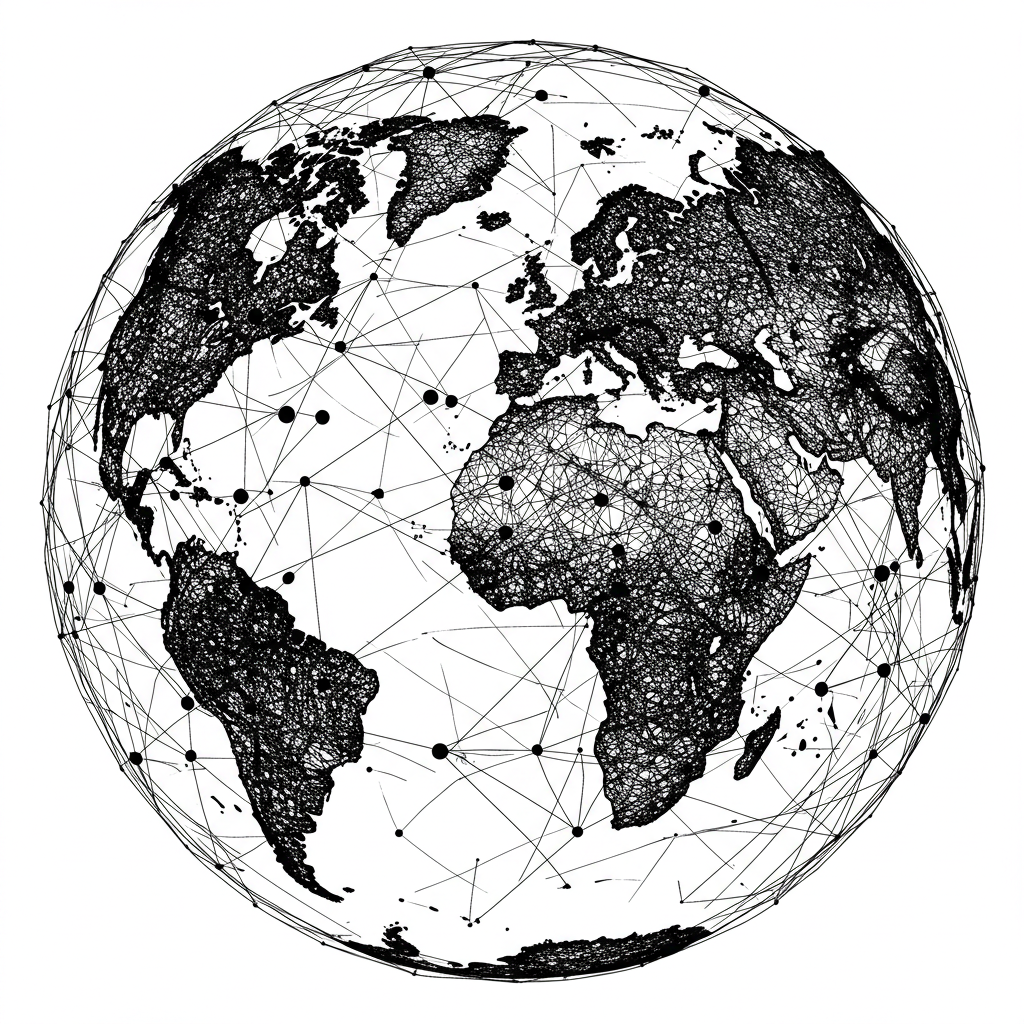
\includegraphics[width=\linewidth]{img/gan.png}
                \caption{{Creata con \href{https://gemini.google.com/}{Gemini}}}
            \end{figure}
    \end{columns}
\end{frame}

\end{document}